\documentclass[10pt,twocolumn,letterpaper]{article}

\usepackage{cvpr}
\usepackage{times}
\usepackage{epsfig}
\usepackage{graphicx}
\usepackage{amsmath}
\usepackage{amssymb}

% Include other packages here, before hyperref.

% If you comment hyperref and then uncomment it, you should delete
% egpaper.aux before re-running latex.  (Or just hit 'q' on the first latex
% run, let it finish, and you should be clear).
\usepackage[breaklinks=true,bookmarks=false]{hyperref}

\cvprfinalcopy % *** Uncomment this line for the final submission

%\def\cvprPaperID{****} % *** Enter the CVPR Paper ID here
%\def\httilde{\mbox{\tt\raisebox{-.5ex}{\symbol{126}}}}

% Pages are numbered in submission mode, and unnumbered in camera-ready
%\ifcvprfinal\pagestyle{empty}\fi
\setcounter{page}{1}
\begin{document}

%%%%%%%%% TITLE
\title{Measuring Heart Rate from Video}

\author{Isabel Bush\\
Stanford Computer Science\\
353 Serra Mall, Stanford, CA 94305\\
{\tt\small ibush@stanford.edu}
}

\maketitle
%\thispagestyle{empty}


%%%%%%%%% ABSTRACT
\begin{abstract}
A non-contact means of measuring heart rate could be beneficial for sensitive populations, and the ability to calculate pulse using a simple webcam or phone camera could be useful in telemedicine. Previous studies have shown that heart rate may be measured in color video of a person's face. This paper discusses the reimplementation of one such approach that uses independent component analysis on mean pixel color values within a region of interest (ROI) about the face. We explore the idea further by assessing the algorithm's robustness to subject movement and bounding box noise and examine new means of choosing the ROI, including segmentation of facial pixels through a reimplementation of GrabCut. Heart rate was measured with an error of 3.4 $\pm$ 0.6 bpm in still video and 2.0 $\pm$ 1.6 bpm in video with movement. Facial segmentation improved the robustness of the algorithm to bounding box noise.

\end{abstract}

\section{Introduction}

A person's heart rate can be indicative of their health, fitness, activity level, stress, and much more. Cardiac pulse is typically measured in clinical settings using electrocardiogram (ECG), which requires patients to wear chest straps with adhesive gel patches that can be abrasive and become uncomfortable for the user. Heart rate may also be monitored using pulse oximetry sensors that may be worn on the fingertip or earlobe. These sensors are not convenient for long-term wear and the pressure can become uncomfortable over time.

In addition to the discomforts of traditional pulse measurement devices, these devices can damage the fragile skin of premature newborns or elderly people. For these populations especially, a non-contact means of detecting pulse could be very beneficial. Non-contact heart rate measurement through a simple webcam or phone camera would also aid telemedicine and allow the average person to track their heart rate without purchasing special equipment. As part of the recent gain in popularity of fitness apps and the quantified self, regular non-obtrusive monitoring through a computer or phone camera may help detect changes in a person's heart rate over time and indicate changing health or fitness. 

Heart rate can be detected without contact through photo-plethysmograpy (PPG), which measures variations in blood volume by detecting changes in light reflectance or transmission throughout the cardiovascular pulse cycle. PPG is usually performed with dedicated light sources with red or infrared wavelengths, as is the case for pulse oximetry sensors. 

Verkruysse \etal showed that the plethysmographic signal could also be detected in video from a regular color camera~\cite{Nelson:2008aa}. They found that the signal could be detected within the red, green, and blue channels of color video of exposed skin, but that it was strongest in the green channel, which corresponds to the fact that hemoglobin has absorption peaks for green and yellow light wavelengths. They also found that although the signal could be detected in multiple locations on the body, it was strongest on the face, especially on the forehead.

Although the plethysmographic signal may be detected in the raw color channel data, it is mixed in with other sources of color variation such as changes in ambient light or motion. Poh \etal found that the signal could be better extracted by using independent component analysis (ICA) to separate independent source signals from the mixed color signals~\cite{Poh:2010aa}.

Other studies have shown that color changes in the face due to pulse may be magnified by amplifying small changes between video frames~\cite{Wu:2012aa}, and that heart rate can be detected through vertical head motion in addition to color changes~\cite{Balakrishnan:2013aa}. Although these are interesting new developments in this space, they are less practical for daily or medical use as the former is more for visualization than quantification, and the latter requires the subject to remain very still for accurate measurements.

In this paper, we explore an approach for heart rate detection using RGB color changes in video of faces similar to that done by Poh \etal~\cite{Poh:2010aa}. In addition to implementing all of the heart rate detection steps from that paper, we also explore improving the selection of pixels used to calculate heart rate including segmenting out the facial pixels through a reimplementation of GrabCut. We examine how these variations on the algorithm compare for still videos as well as when there is movement or noise in the videos.

The rest of this paper details the process used to measure heart rate from video of a person's face. Section \ref{tech_approach} details the technical approach, section \ref{exp_setup} discusses the experimental setup, section \ref{results} reveals the results, and section \ref{conclusion} offers some conclusions.

\section{Technical Approach} \label{tech_approach}

Detecting heart rate in video consists of three main steps. First, the facial region must be detected in each frame of the video since the face is the only portion of the frame that will contain heart rate information. Second, the desired region of interest (ROI) within the face bounding box must be chosen. And third, the plethysmographic signal must be extracted from the change in pixel colors within the ROI over time and analyzed to determine the prominent frequency within the heart rate range.

\subsection{Face Detection and Tracking}

\begin{figure}
\begin{center}
	\includegraphics[scale=0.7]{figures/haar}
\end{center}
\caption{Example Haar-like features used in the boosted cascade face classifier from the original paper by Viola and Jones~\cite{Viola:2001aa}. Each feature is calculated as the sum of pixels in the grey rectangles less the sum of pixels in the white rectangles.}
\label{haar}
\end{figure}

Face detection and tracking is performed using Haar cascade classifiers as proposed by Viola and Jones~\cite{Viola:2001aa} and improved by Lienhart \etal~\cite{Leinhart:2002aa}. Specifically, we use the OpenCV Cascade Classifier pre-trained on positive and negative frontal face images~\cite{opencv_library}. The face detector is built from a cascade of classifiers of increasing complexity, where each classifier uses one or more Haar-like features.

The features consist of two, three, or four rectangular pixels as shown in figure \ref{haar}. Each feature is calculated as the sum of pixels in the grey rectangles less the sum of pixels in the white rectangles. These features are able to detect simple vertical, horizontal, and diagonal edges and blobs. 

Since there are over 180,000 potential features in each sub-window, only a small subset of these features are actually used. The AdaBoost learning algorithm is used to train classifiers built on one to a few hundred features. To choose which feature(s) to use, a weak classifier is trained on each feature individually and the classification error is evaluated. The classifier (and associated feature) with the lowest error is chosen for that round, the weights are updated, and the process is repeated until the desired number of features are chosen. This process creates a single strong classifier that is a weighted combination of numerous weak classifiers.

The strong classifiers are then used in series in the attentional cascade, which is essentially a decision tree for each sub-window within the image. The cascade begins with a simple classifier (built on a single feature) with a low threshold such that it is designed to have a very low false negative rate (with high false positive rate). If this classifier yields a positive result on a window, that window passes to the next classifier. If the classifier yields a negative result, the sub-window is rejected. Each round of the cascade uses a more complicated classifier built on more and more features since it must differentiate sub-windows that all passed the previous round. But since there are fewer windows in each round, the processing time is less than if the complicated classifiers were used on all windows in the image.

To achieve invariance with respect to lighting and scale, sub-windows are normalized and the final detector is slid over the image at varying window sizes. Any overlapping positive-classification windows are averaged to create a single facial bounding box.

This face detection algorithm is applied to each frame in the video and outputs a bounding box for each face it detects. To maintain consistency across frames, if no face is detected in a frame, the face from the previous frame is used, and if multiple faces are detected, the face nearest to that in the previous frame is used. 

\subsection{Region of Interest Selection}

Since the face bounding box found using face detection contains background pixels in addition to the facial pixels, an ROI must be chosen from within the bounding box. The simplest choice of ROI is to use the center 60\% of the bounding box width and the full height, as was done by Poh \etal~\cite{Poh:2010aa}. Since the bounding box is usually within the face region height-wise but outside the face width-wise, this method simply adjusts the box to exclude background pixels to the sides of the face. With this method, some hair or background pixels are usually still present at the corners of the box. 

We also explore other means of selecting the ROI. We examine the effects of removing the eye region, which contains non-skin pixels that may vary across frames due to blinking or eye movement. Removing pixels from between 25\% and 50\% of the bounding box height worked well to remove the eyes. We also explore retaining only the pixels above the eye region, since Verkruysse \etal found the forehead has the strongest plethysmographic signal. Finally, we explore segmenting out the facial pixels from the background pixels.

Facial segmentation is performed using GrabCut, developed by Rother \etal~\cite{Rother:2004aa}. GrabCut segments images by iteratively minimizing an energy cost function. This energy minimization can be achieved by defining a graph model to represent the image and determining the minimum cut for the graph to yield two sets of nodes, which represent the foreground and background pixels of the image. Although an implementation of GrabCut is available in the OpenCV library~\cite{opencv_library}, the algorithm was also reimplemented as part of this project to better understand how it works.

The graph model is formed by assigning a node for each pixel in the image. Edges are formed between neighboring image pixels, with weights defined by the color similarity between the two pixels. More similar pixels have higher edge weights to encourage them to end up in the same set after the graph cut. Each pixel has eight neighbors, and the edge weights between them are calculated as

$$ W_N(p,q) = \frac{\gamma}{dist(p,q)} * e^{-\beta ||z_p-z_q||^2}$$ 
where $z_p$ is the color of pixel p, $dist(p,q)$ is the pixel distance between p and q, and the constants are set to $\gamma = 50$ and 
$$\beta = \frac{1}{2 \langle ||z_p-z_q||^2\rangle}$$
following Boykov and Jolly~\cite{Boykov:2001aa}.

Two more nodes are added to the graph and connected to all other nodes. These nodes represent the foreground and background portions of the image and will be placed in opposite sets by the min-cut algorithm. The weights of the terminal edges between a pixel and the foreground and background nodes represent the probability that the pixel belongs to each set. These probabilities are determined using Gaussian Mixture Models (GMMs) for the foreground and background pixel color distributions.

The foreground set is initialized to contain all pixels inside the bounding box and the background set is initialized to contain all pixels outside the bounding box. Pixels outside the box are assumed to be certainly background pixels, while pixels within the bounding box are potentially foreground or background. In each iteration of GrabCut, GMMs are formed for both the foreground and background sets and pixels in those sets are assigned to one of the $K$ GMM clusters. The GMMs were determined using the scikit-learn library~\cite{scikit-learn}.

The terminal weights for all uncertain pixels $p$ are then calculated as

$$W_T(p) = - log \sum_{i=1}^K \pi_i \frac{1}{\sqrt{det(\Sigma_i})} e^{(-\frac{1}{2}[z_p-\mu_i]^T \Sigma_i^-1 [z_p - \mu_i])}$$
where the summation is over the $K$ GMM clusters in either the foreground or the background GMM, $\mu_i$ and $\Sigma_i$ are the mean and covariance of the $i^{th}$ cluster, and $\pi_i$ is the fraction of the model's pixels assigned to the cluster. The foreground GMM is used to calculate the edge weights to the background terminal node, and vice versa. For any certain background pixels $p$ (outside the original bounding box), we set $W_T(p) = 0$ for the edge to the foreground node and $W_T(p) = 8\gamma + 1$ for the edge to the background node, which ensures these pixels are assigned to the background set by the min-cut algorithm.

Once all edge weights are defined, a minimum s-t cut may be made between the terminal nodes to define the new background and foreground sets for that iteration. The minimum graph cut was found using the PyMaxflow Python library built on top of Vladimir Kolmogorov's C++ GraphCut implementation~\cite{Boykov:2004aa}.

Since GrabCut assumes that the pixels outside of the bounding box are certainly background pixels and pixels within the bounding box are potentially foreground or background pixels, we must modify the bounding box found in face detection. To ensure the bounding box includes all face pixels but excludes some hair pixels (so that hair will be considered as background), a bounding box that was 80\% of the original box width and 120\% of the original box height worked well as input to GrabCut.

\subsection{Heart Rate Detection}

Once we have an ROI for each frame, we can begin to extract the heart rate from the color image data. The first step is to average the pixels in the ROI across each color channel to get three signals $x_R(t)$, $x_G(t)$, and $x_B(t)$ corresponding to the average red, green, and blue facial pixels at time $t$. We then normalize these signals across a 30-second sliding window with a 1-second stride (so the heart rate is re-estimated every second).

We then use ICA to extract the independent source signals from the observed mixed color signals. ICA assumes that the number of source signals is no more than the number of observed signals, so we assume there are three source signals $s_1(t)$, $s_2(t)$, and $s_3(t)$ contributing to the observed color changes in the three channels. ICA assumes the observed mixed signals are a linear combination of these source signals. Although this assumption may not be valid as changes in blood volume and the intensity of reflected light in skin tissue over distance may be nonlinear, for the 30-second time window it should be a reasonable approximation. With this linear approximation for signal mixing, we have 
	$$x(t) = As(t)$$ 
	$$s(t) = A^{-1}x(t)$$
where $x(t) = [x_R(t)\ x_G(t)\ x_B(t)]^T$, $s(t) = [s_1(t)\ s_2(t)\ s_3(t)]^T$, and $A$ is a 3x3 matrix of coefficients. Then ICA attempts to find an approximation of $A^{-1}$ that maximizes the non-Gaussianity of each source. We can use FastICA from the scikit-learn library to recover the approximate source signals $s(t)$~\cite{scikit-learn}.

Once we have the source signals, we can apply a Fourier transform to the data to examine their power spectrum and determine the prominent signal frequencies. We can isolate frequency peaks in the power spectrum within the range 0.75 to 4 Hz, which corresponds to physiological heart rate ranges of 45 to 240 bpm. The measured heart rate will be the frequency within the acceptable range corresponding to the peak with the highest magnitude.

\section{Experimental Setup} \label{exp_setup}

\begin{figure}
\begin{center}
	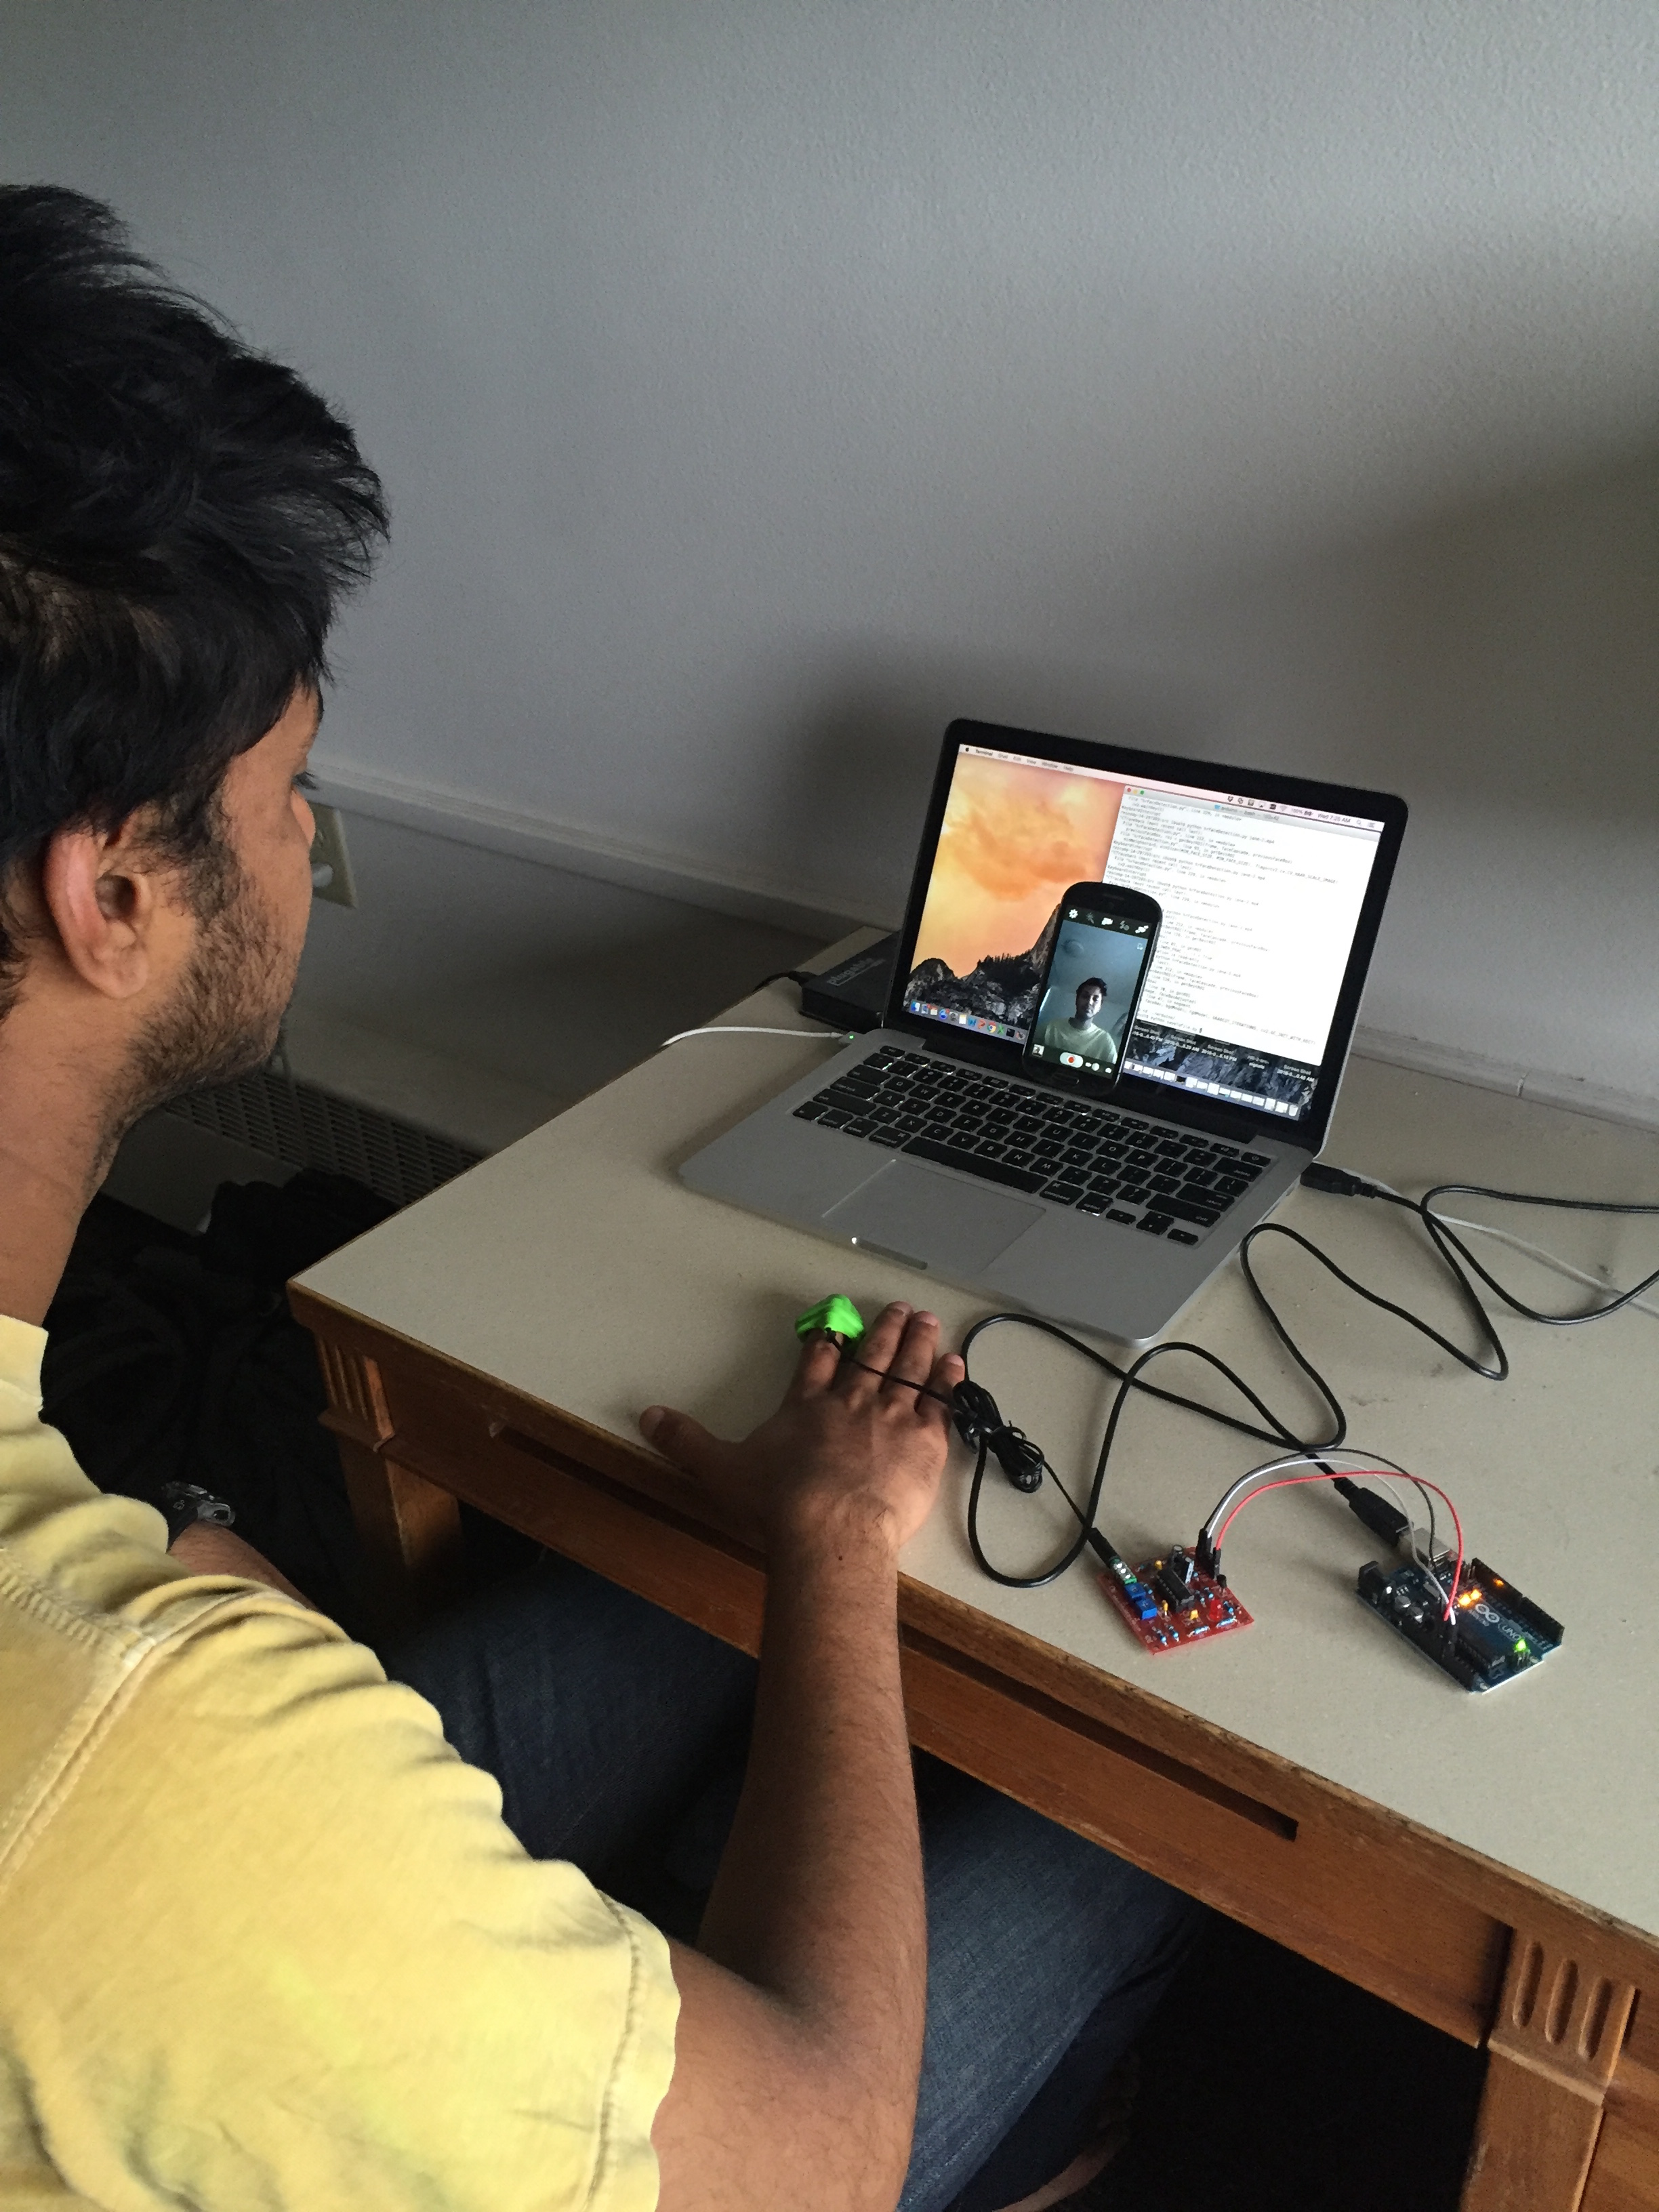
\includegraphics[scale=0.045]{figures/setup}
	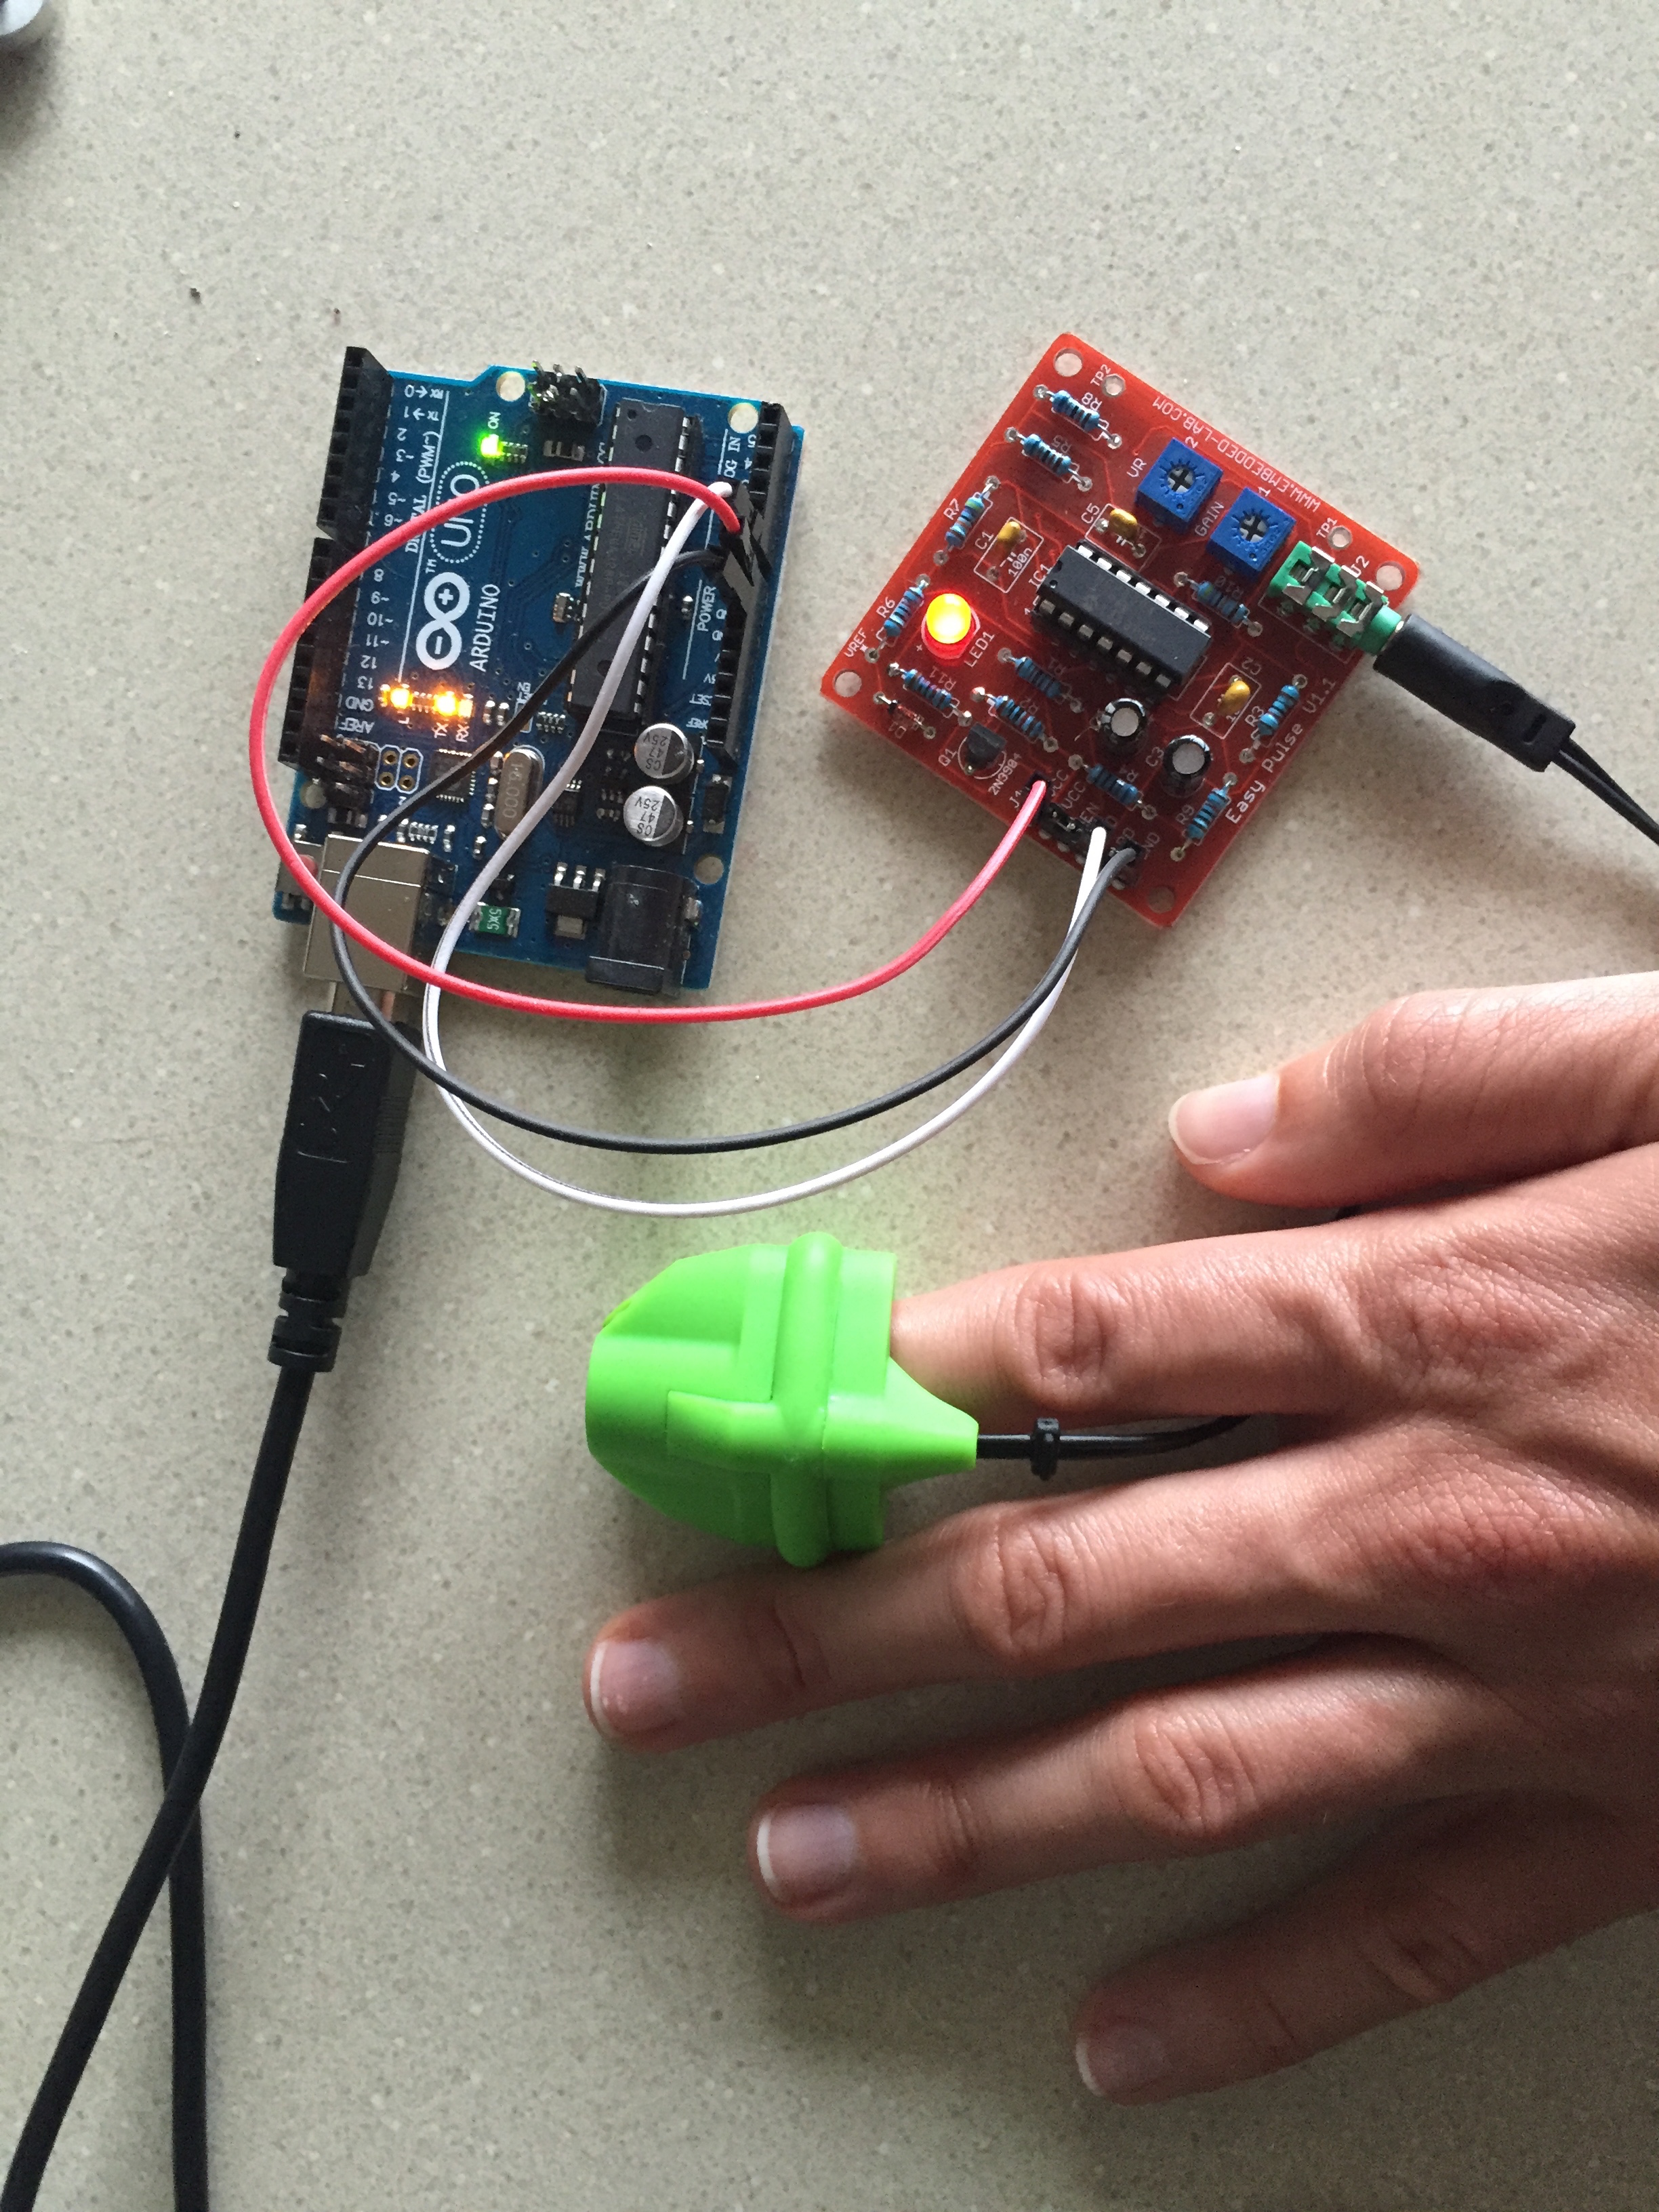
\includegraphics[scale=0.045]{figures/ref_setup}
\end{center}
\caption{Experimental setup. One-minute videos of a subject's face were captured with a Samsung camera, and a reference PPG signal was recorded using the Easy Pulse fingertip PPG sensor and an Arduino Uno.}
\label{setup}
\end{figure}

One-minute videos were collected of 10 subjects with varying skin-tones and in varying lighting conditions, including both natural and artificial light. Videos were taken with a Samsung SGH-i437 phone front-facing camera and saved in mp4 format. Video frames had a resolution of 480 x 640 pixels and were captured at 14.99 fps. At least two videos of each subject were taken, one with the subject remaining as still as possible and one in which the subject moved slightly (tilting, turning, and shifting their facial position within the frame). 

The recording setup is shown in figure \ref{setup}. During video recording, subjects wore a finger PPG sensor so that the heart rate results from the video could be compared to a ground truth. The PPG sensor used was an Easy Pulse hobbyist sensor from Embedded Lab~\cite{Bhatt:aa}. It uses an HRM-2511E sensor to measure infrared light transmission through the fingertip and output the analog PPG signal. This signal was fed into the analog-to-digital convertor on the Arduino Uno micro-controller and sampled at 200 Hz. The sampled signal was then processed in the same manner as the ICA source signals from the video heart rate detection approach. The highest peak within the power spectrum of the signal was taken to be the reference heart rate for each 30-second window.

In addition to determining the robustness of the algorithm to subject movement, we also examine the robustness to bounding-box noise. Although the bounding box was usually well centered on the face in each frame, we could imagine that in a noisier environment in which there is more movement of either the camera or subject, poorer lighting, facial occlusions, or more background clutter, there could be more error in the location of the facial bounding box. To simulate this, we can add artificial noise to the bounding box corner locations found with the Haar cascade classifier. In each frame, corners of the bounding box were shifted horizontally and vertically by percentages of the width and height, where the percentages were chosen uniformly at random up to a maximum noise percentage. This maximum noise percentage varied from 0 to 50\% of the bounding box size.

\section{Results} \label{results}

The sections below detail the experimental results. Section \ref{step_results} shows some qualitative results from each step of the algorithm. Section \ref{hr_acc} shows the algorithm accuracy as compared to the reference signal for video of both still and moving subjects. Section \ref{robust_noise} discusses the heart rate accuracy when varying amounts of noise is added to the facial bounding box.

\subsection{Algorithm Step Results} \label{step_results}

\begin{figure}
\begin{center}
	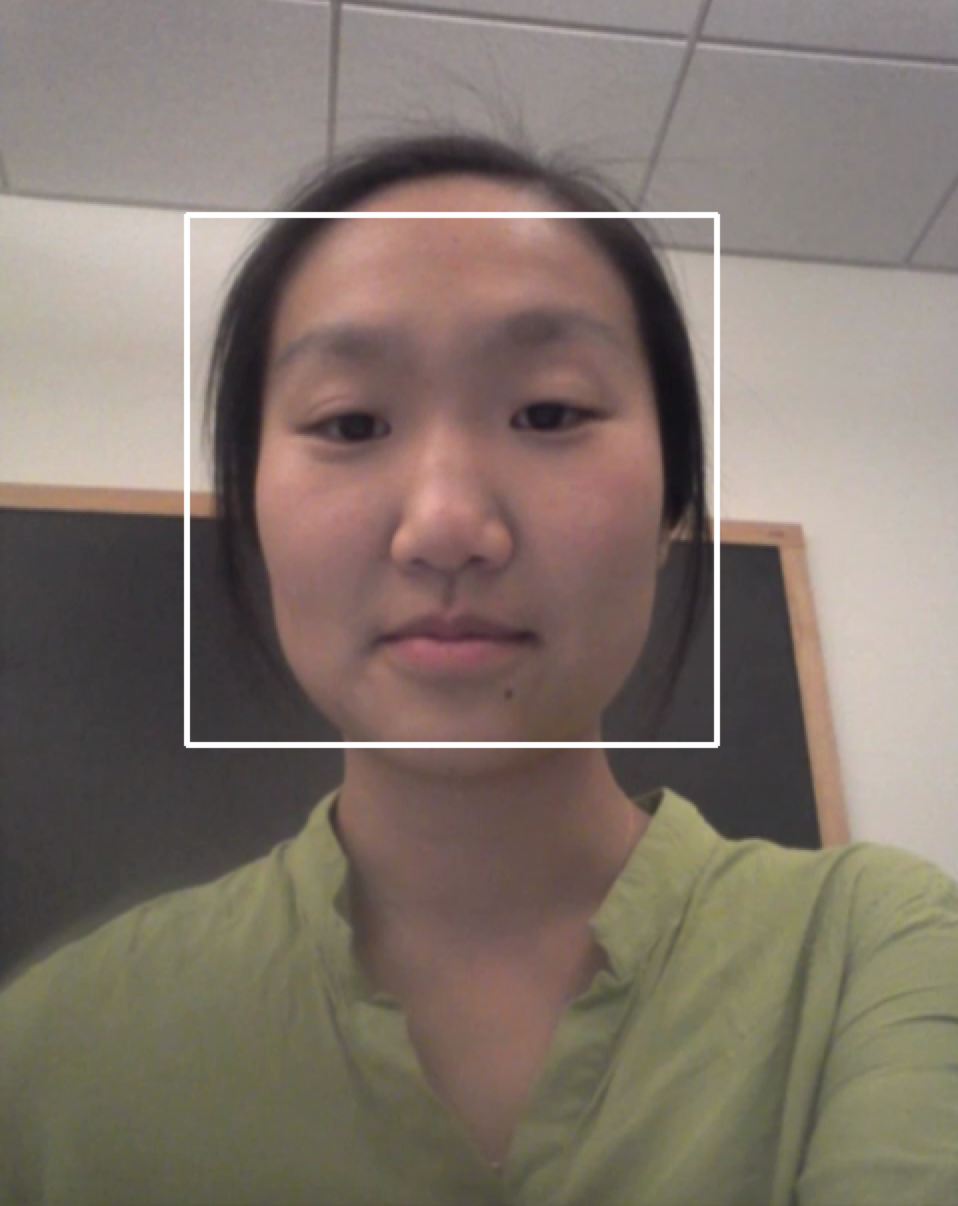
\includegraphics[scale=0.3]{figures/jane_bb}
\end{center}
\caption{A facial bounding box.}
\label{face_bb}
\end{figure}

\begin{figure}
\begin{center}
	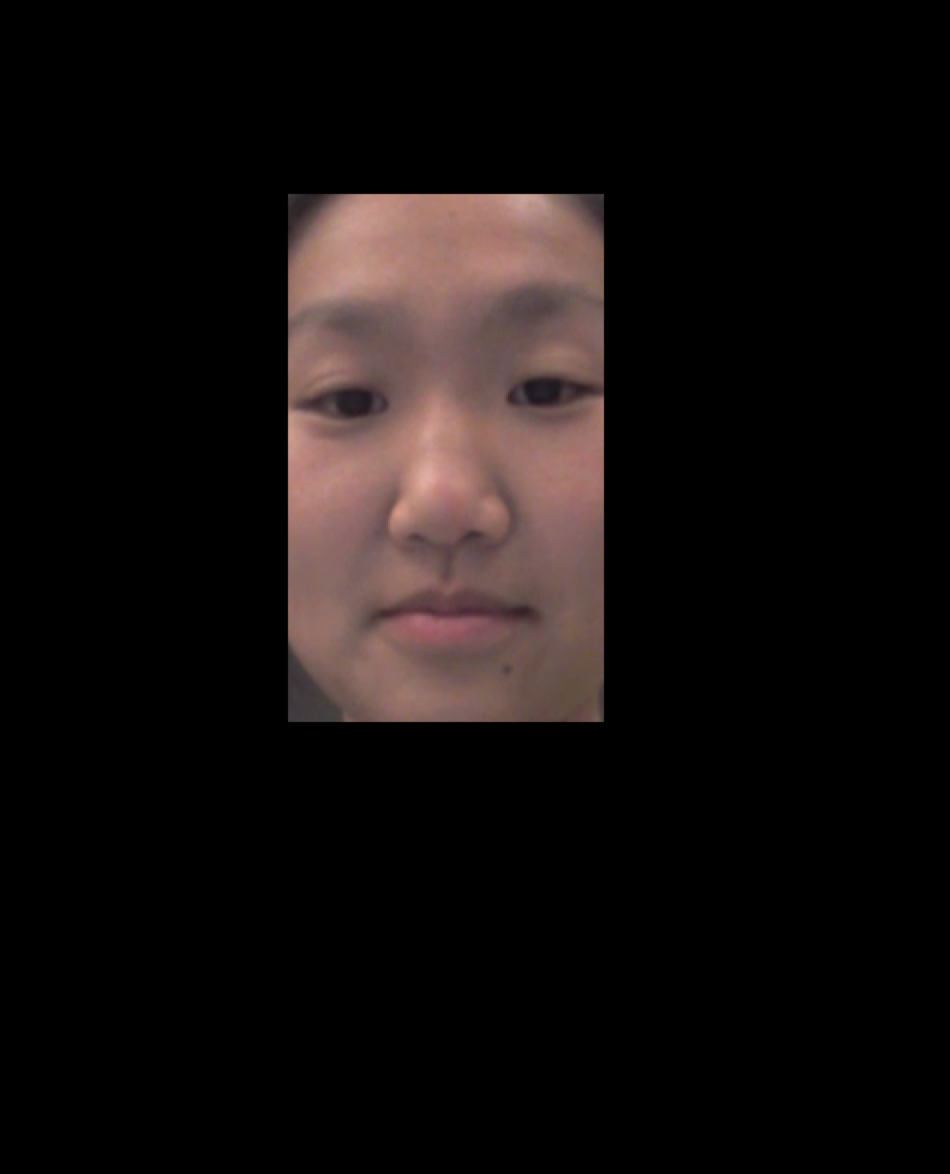
\includegraphics[scale=0.2]{figures/jane_box}
	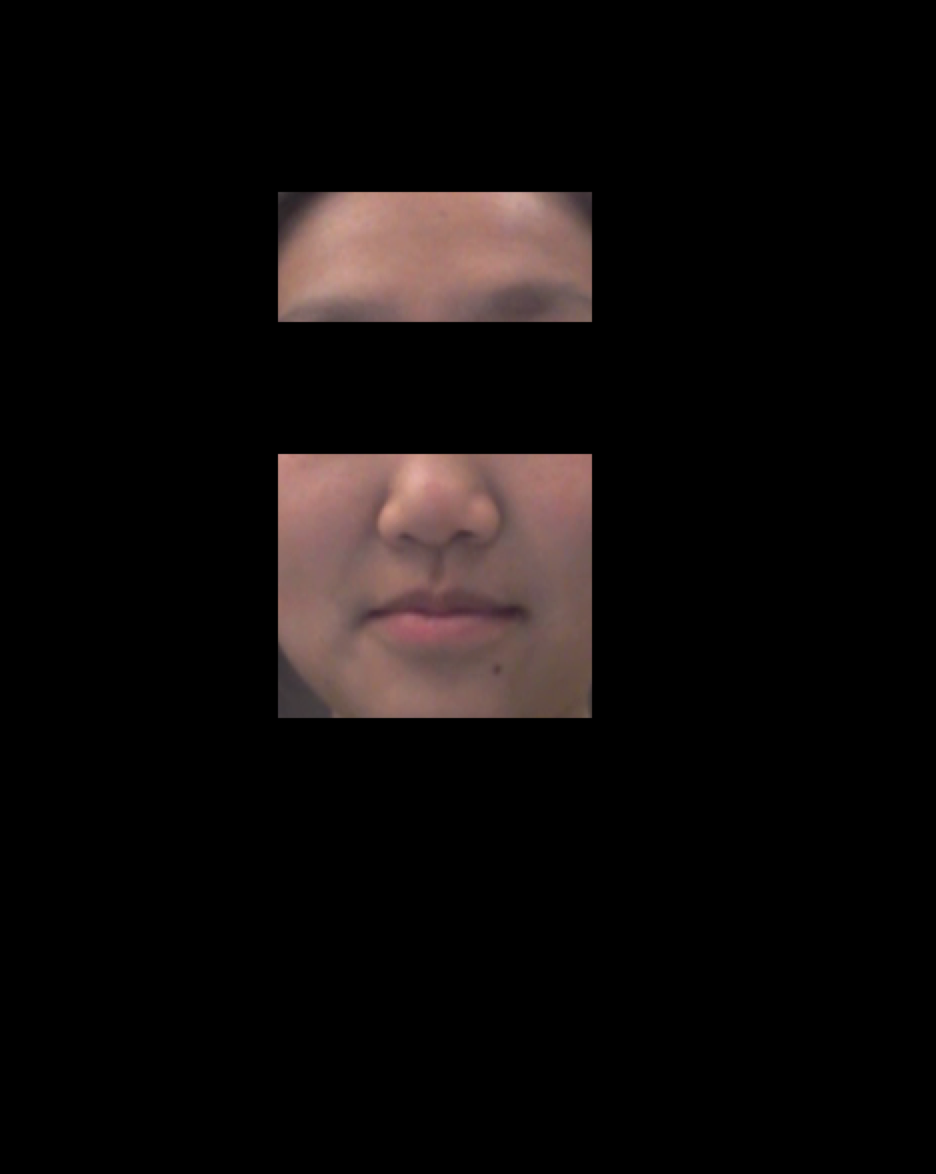
\includegraphics[scale=0.2]{figures/jane_no_eyes}
	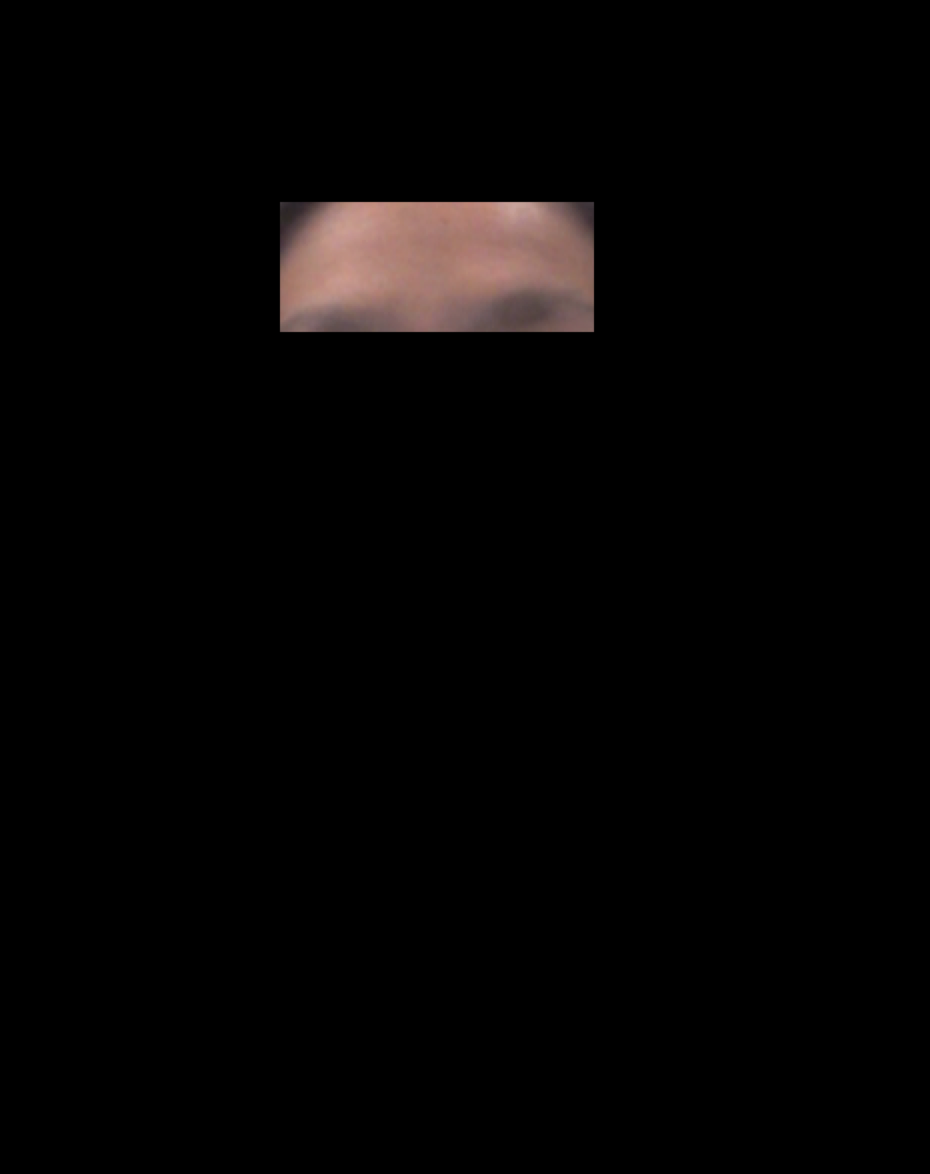
\includegraphics[scale=0.2]{figures/jane_forehead}
	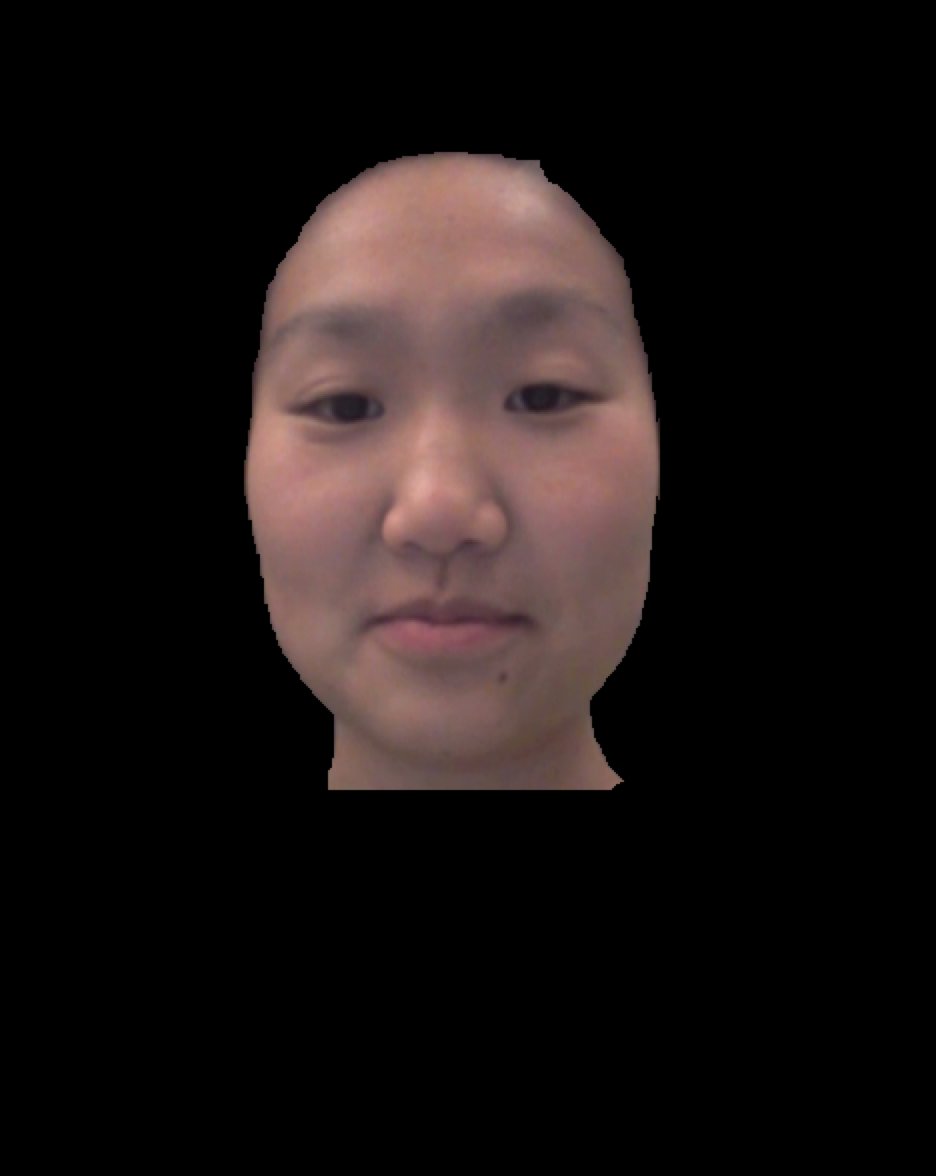
\includegraphics[scale=0.2]{figures/jane_segment}
\end{center}
\caption{Various ROIs used to calculate heart rate including a narrower bounding box, a box with the eyes removed, the forehead region, and segmented facial pixels.}
\label{roi}
\end{figure}

Once the facial bounding box(es) found using the Haar cascade classifiers were narrowed down to a single bounding box on the subject's face, the box accurately located the face in nearly all video frames, as in figure \ref{face_bb}. 

Results of various ROI selection options, including a narrower box, a box with the eyes removed, a box around the forehead, or a segmented face, may be seen in figure \ref{roi}. The simplest ROI, namely the narrower bounding box that was used by Poh \etal, usually contained mostly skin pixels for frontal images, although there was also sometimes hair or background appearing at the corners. When the subject tilted or turned their head, more background pixels become part of the ROI, as shown in figure \ref{tilt_turn}.

Figure \ref{segment} shows the original bounding box, adjusted bounding box, and segmentation results for a straight face using the reimplementation of GrabCut. As can be seen, the segmentation excludes most hair and background pixels within a couple iterations. This seems especially useful when the subject twists or turns as in figure \ref{tilt_turn} as it removes the variability in background pixels that was present using the simple narrow bounding box ROI.

\begin{figure}
\begin{center}
	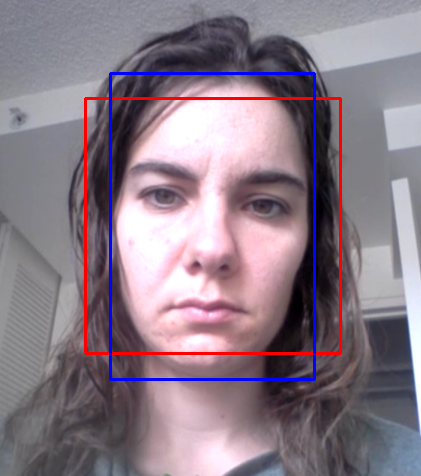
\includegraphics[scale=0.25]{figures/segment_bb}\\
	
\includegraphics[scale=0.25]{figures/my_seg_it1}
	
\includegraphics[scale=0.25]{figures/my_seg_it2}
\end{center}
\caption{The original bounding box in red and adjusted bounding box that was input into the GrabCut segmentation algorithm in blue (top) as well as the first two iterations of the GrabCut implementation (bottom).}
\label{segment}
\end{figure}

\begin{figure}
\begin{center}
	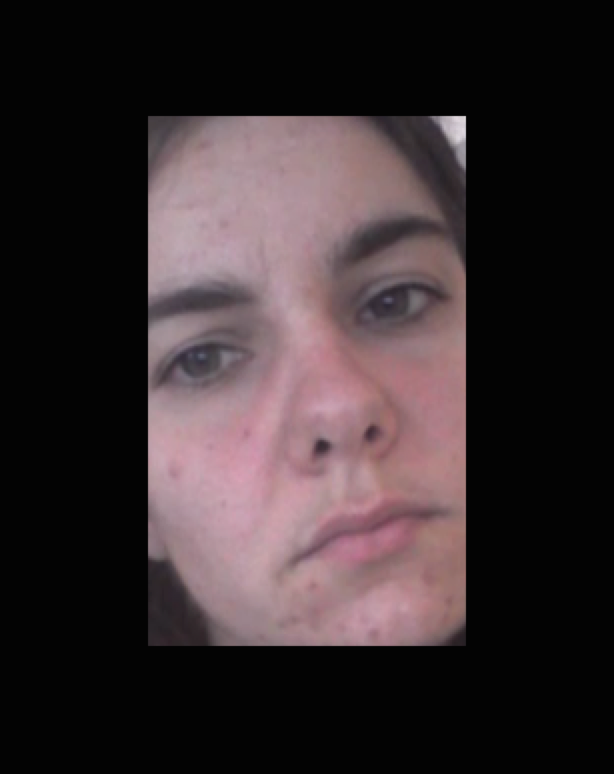
\includegraphics[scale=0.25]{figures/tilt_bb}
	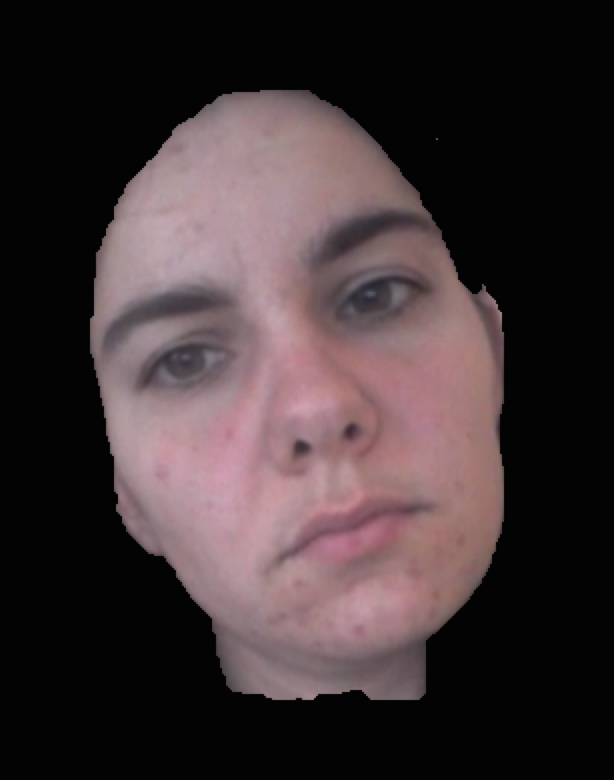
\includegraphics[scale=0.25]{figures/tilt_segment}\\
	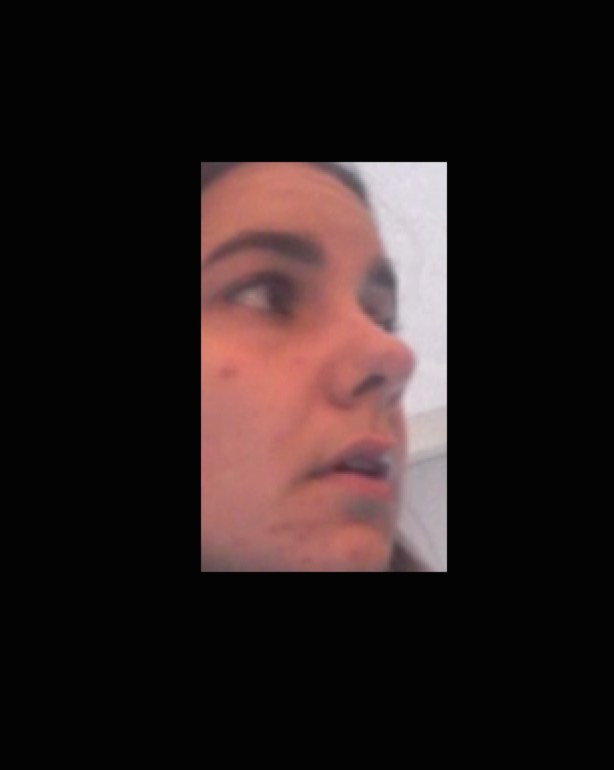
\includegraphics[scale=0.25]{figures/turn_bb}
	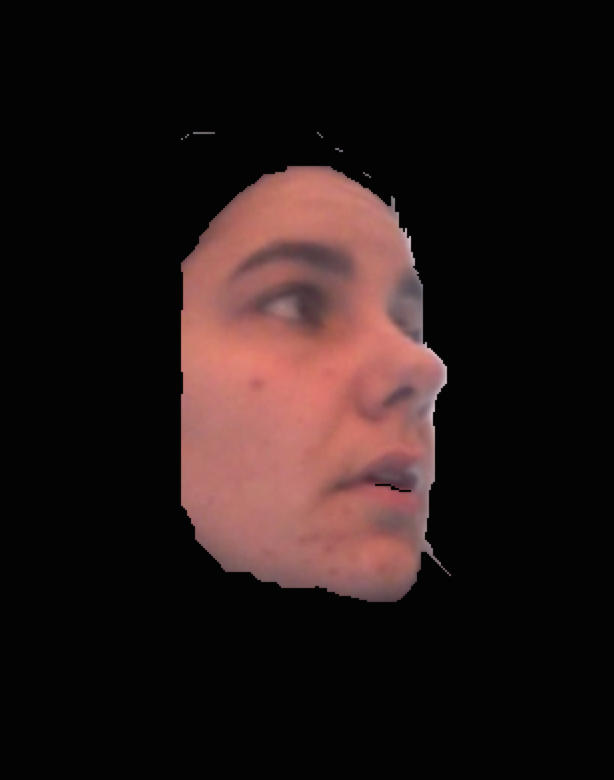
\includegraphics[scale=0.25]{figures/turn_segment}
\end{center}
\caption{Comparison of ROI selection for tilted and turned faces using a narrower bounding box (left) versus facial segmentation (right). The segmentation does a better job of eliminating the background pixels.}
\label{tilt_turn}
\end{figure}

The next step of the algorithm is to find the heart rate from the selected ROI pixels. As described in the technical approach, this process included finding the mean RGB pixel values within the ROI for each frame and then normalizing across a 30-second window, ICA to extract independent source signals, and power spectrum analysis to determine the prominent frequencies.

Figure \ref{time_plots} shows the normalized mean pixel intensity for the three color channels as well as the three source signals found through ICA for a 10-second portion of a window. Figure \ref{freq_plot} shows the power spectra for the three source signals within the physiological heart rate range. The strongest frequency in this range corresponds to the heart rate reading for this time-step.

\begin{figure}
\begin{center}
	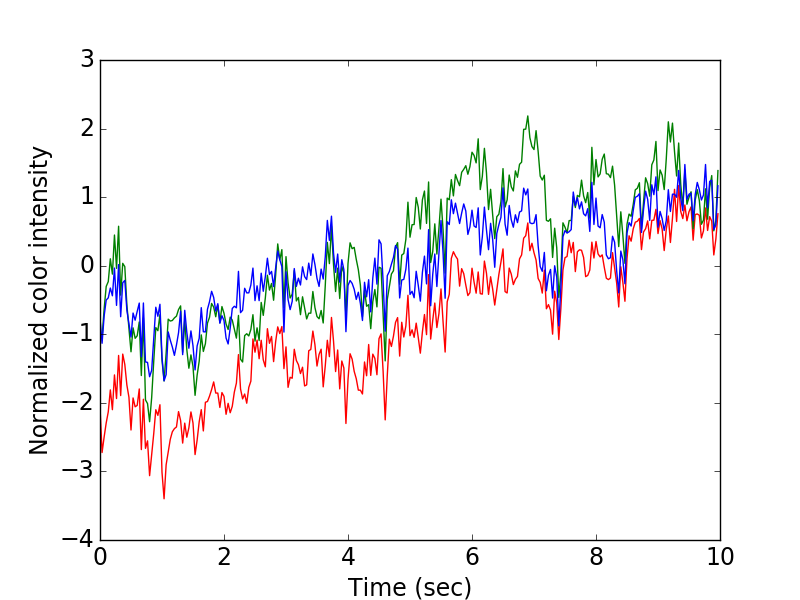
\includegraphics[scale=0.46]{figures/RGB_signals_10sec.png}
	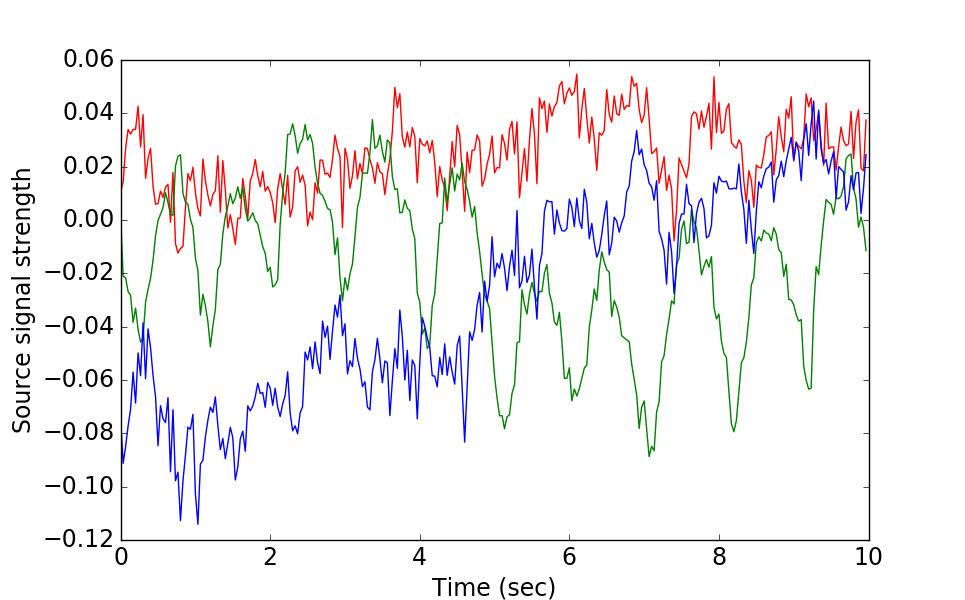
\includegraphics[scale=0.38]{figures/src_signals_10sec.png}
\end{center}
\caption{Example mean RGB color channel pixel values within the ROI (top) and associated source signals found through ICA (bottom). The source signal shown in green appears to oscillate at approximately 1 Hz and corresponds to the subject's pulse. }
\label{time_plots}
\end{figure}

\begin{figure}
\begin{center}
	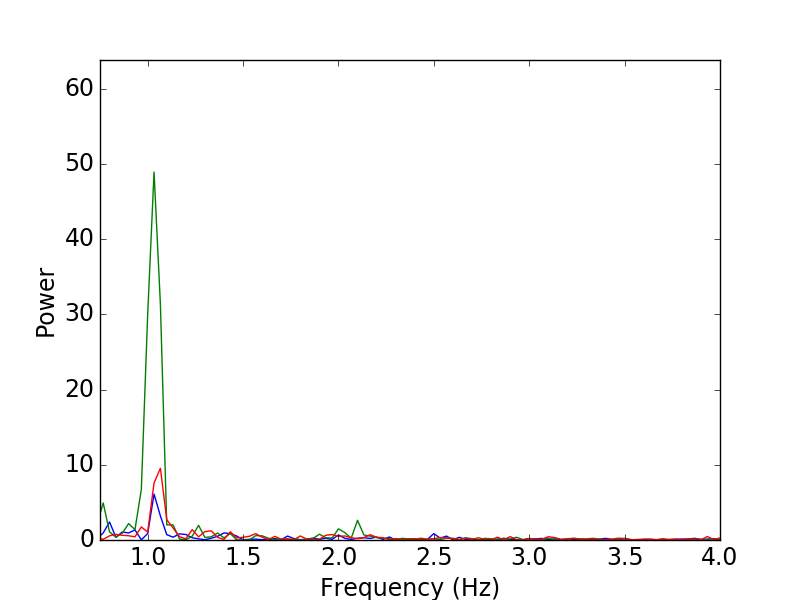
\includegraphics[scale=0.48]{figures/spectrum_10sec.png}
\end{center}
\caption{Example power spectra for three source signals over the physiological heart-rate range. The prominent frequency (0.97 Hz) corresponds to the heart-rate measurement of 58 bpm for this time-step.}
\label{freq_plot}
\end{figure}

\subsection{Heart Rate Accuracy} \label{hr_acc}

\begin{figure}
\begin{center}
	\includegraphics[scale=0.6]{figures/still_move_error.png}
\end{center}
\caption{Heart rate error for videos of still faces and videos with movement, calculated using inlier measurements (within 10\% of the reference measurement) for each of the four ROI choices.}
\label{still_move_error}
\end{figure}

\begin{figure}
\begin{center}
	\includegraphics[scale=0.48]{figures/still_move_outliers.png}
\end{center}
\caption{Percentage of heart rate measurements that are outliers for videos of still faces and videos with movement, calculated using each of the four ROI choices. More outliers are seen for videos with movement and when only the forehead region is used as the ROI.}
\label{still_move_outliers}
\end{figure}

For videos of still faces, the calculated heart rate error was 3.4 $\pm$ 0.6 bpm. For videos of subjects tilting, turning, and shifting their faces, the calculated heart rate error was 2.0 $\pm$ 1.6 bpm. These errors were calculated using only inlier measurements, which were defined to be measurements within 10\% of the reference heart rate. Any outliers indicate that the algorithm most likely failed to pick up the pulse as one of the ICA source signals and thus chose some other signal as the dominate frequency. These outlier measurements may be any random frequency within the allowable range and thus including them in the mean and standard deviation calculations does not indicate how closely the algorithm matches the reference heart rate. Using only inlier measurements, the errors were consistent for all ROI selection methods, as seen in figure \ref{still_move_error}. 

The number or percentage of outlier measurements, however, does provide a good indicator of the robustness of the algorithm as any outlier indicates a failure of the algorithm to find the heart rate in that window. For each one-minute video, 30 heart rate measurements were calculated (30-second windows with a 1-sec stride). The percentage of these 30 measurements that were outliers may be seen in figure \ref{still_move_outliers}. Approximately 4\% of measurements are outliers for videos of still faces and 17\% are outliers for videos with movement. The simple narrower bounding box ROI, a box with the eyes removed, and a segmented ROI all perform about equally, whereas we see that just using the forehead increases the number of outliers. This is likely because if only the forehead region is used, there are fewer facial pixels to diminish the effects of any hair pixels that may be included in the ROI.

\subsection{Robustness to Noise} \label{robust_noise}

\begin{figure}
\begin{center}
	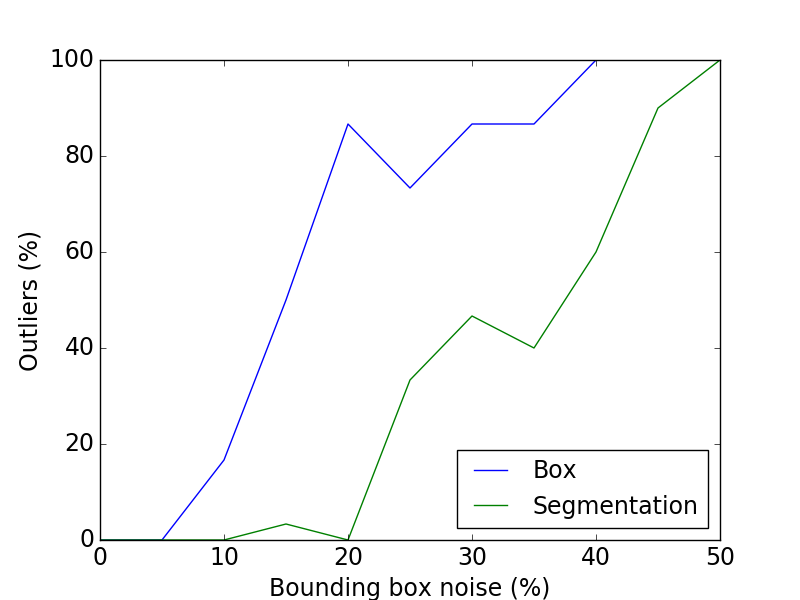
\includegraphics[scale=0.4]{figures/bb_noise_outliers.png}
\end{center}
\caption{Percentage of measurements that are outliers as a function of the maximum bounding box noise introduced in each frame (as a percentage of the true bounding box size) for a video of a still face. As expected, the number of outliers increases with the amount of noise, but a segmented ROI is more robust to handling this noise than a narrow box ROI.}
\label{noise_outliers}
\end{figure}

We can also measure robustness of the algorithm to bounding box noise by artificially introducing random noise of varying magnitude to the facial bounding box found in the first step of the algorithm. Figure \ref{noise_outliers} shows the percentage of measurements that were outliers as a function of the maximum magnitude of introduced noise. As can be seen, using a segmented ROI rather than simply the narrower box helps to mitigate the effects of increasing bounding box noise. A narrow box ROI has over 50\% outliers with less than 20\% bounding box noise, while the segmented ROI is still near zero outliers at 20\% and does not climb above 50\% outliers until near 40\% bounding box noise.

\section{Conclusion} \label{conclusion}

We have seen that heart rate may be measured in regular color video of a person's face. We observed heart rate errors of 3.4 $\pm$ 0.6 bpm for videos of still faces and 2.0 $\pm$ 1.6 bpm for videos with movement. Since the calculated heart rate was consistently lower than the reference in all videos and with small standard deviation, it is possible that the base error is due to a miscalculation in video frame rate or finger pulse sensor sample rate. If the Samsung camera had a frame rate that was 5\% higher than the reported frame rate, or if the Arduino sample rate was actually 5\% lower than desired, or if there were a smaller error in both rates, this would account for the observed heart rate calculation errors. Future studies could use a medical-grade pulse monitor to ensure that the reference heart rate is as accurate as possible. If it is determined that there is truly always a consistent offset between the reference and the calculated heart rate as observed in this study, a calibration step could be used to remove the bias. Such a system could potentially measure heart rate in still video to within 0.6 bpm. 

Although sample rate errors could cause a consistent bias in heart rate measurements, the standard deviation and percentage of outlier measurements provide a better indication of the robustness of the algorithm to changes in the video. We observed under 5\% outlier measurements for still faces and under 20\% for videos of moving faces. Since these are both well under 50\%, outliers could be easily identified and removed from heart rate calculations even if there were no reference heart rate to use as a basis. We also found that as bounding box noise increased, choosing an ROI by segmenting out facial pixels helped to diminish the noise effects and keep the outliers low.

Overall we find that for clean videos of subject's faces in good lighting, using a simple ROI defined by 60\% of the width and the full height of the facial bounding box works just as well as removing the eye region or segmenting out facial pixels, and outperforms a box only around the forehead region. Since this simple box ROI is much faster than performing GrabCut to segment out the facial pixels (more than 12 times as fast), the simple box would be the suggested method for such videos.

However, if the bounding box is expected to be noisy, segmentation is a good method to remove some of this noise and maintain accurate measurements. Future studies could involve taking video in low-light and with a cluttered background or with occlusions or multiple subjects in the frame to quantify how much bounding box noise is realistically present in such situations. This could help to determine if segmentation is necessary.

Another future study could attempt to do video heart rate calculations in real-time rather than with pre-recorded videos. Currently, using a simple box ROI, a one-minute video may be processed on a MacBook Pro (2.6 GHz) in under two minutes, processing about 8 fps. This may in fact already be fast enough for real-time if a camera with a frame rate under 8 fps were used to record the videos. Since the maximum physiological heart rate expected by the algorithm is 4 Hz, the sample rate would be just enough to avoid aliasing at 8 fps (8 Hz is the Nyquist frequency). Since 4 Hz is a highly unlikely heart rate especially for a person at rest, the frame rate could likely be decreased even further and the algorithm max heart rate adjusted accordingly. If segmentation is required (for example if there is significant bounding box noise), other adjustments would be required to speed up the algorithm processing time.

%-------------------------------------------------------------------------------
\newpage

{\small
\bibliographystyle{ieee}
\bibliography{egbib}
}

\end{document}
